%&"../virtual"

\begin{document}
    \title{虚拟机网络性能测试}
    \maketitle
    \section*{要求}
    Virtualized and bare metal network performance test.
    \begin{itemize}
        \item Download QEMU 5.2.0 from \href{https://www.qemu.org/download/}{https://www.qemu.org/download/} and compile.
        \item Create 2 VMs with TAP mode network (e1000 and virtio-net) by QEMU.
        \item Connect to your VM through VNC viewer or SSH.
        \item Compare the network performance of your host machine and VMs.
    \end{itemize}
    \section{编译 QEMU}
    使用 QEMU 5.2.0 (Dec 8th 2020),为了方便后续的版本对比,根据说明文档\cite{readme}直接克隆存储库。根据官方的 wiki 说明\cite{installwiki},需要安装一些额外包。通过下面的脚本进行下载、编译:
    \code[language=bash]{INSTALL.sh}
    其中 \verb"libvte-2.90-dev" 包已经被废弃。编译如图 \ref{fig:compile} 所示成功,安装如图 \ref{fig:install} 所示成功。
    \begin{figure}[h]
        \centering
        \begin{minipage}{0.48\textwidth}
            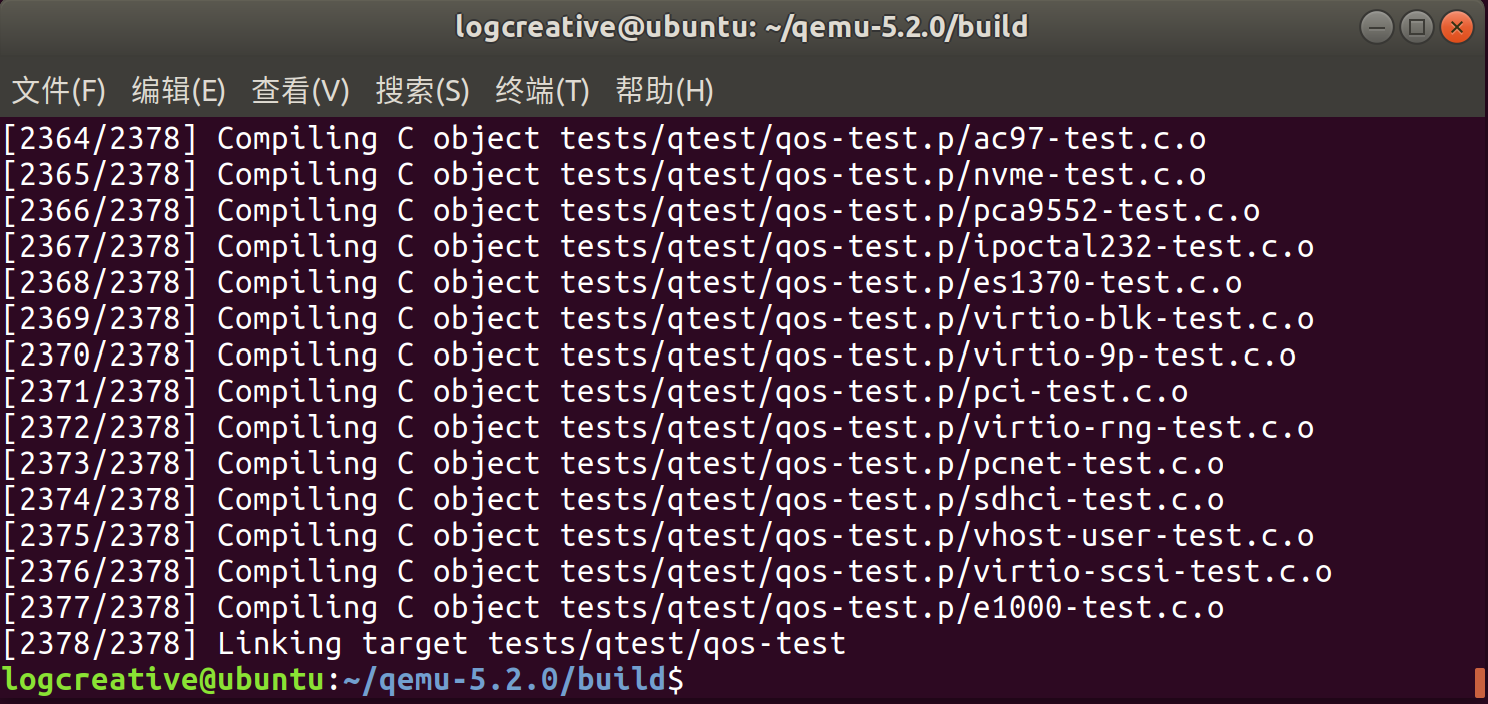
\includegraphics[width=\linewidth]{compile}
            \caption{QEMU 编译}\label{fig:compile}
        \end{minipage}
        \begin{minipage}{0.48\textwidth}
            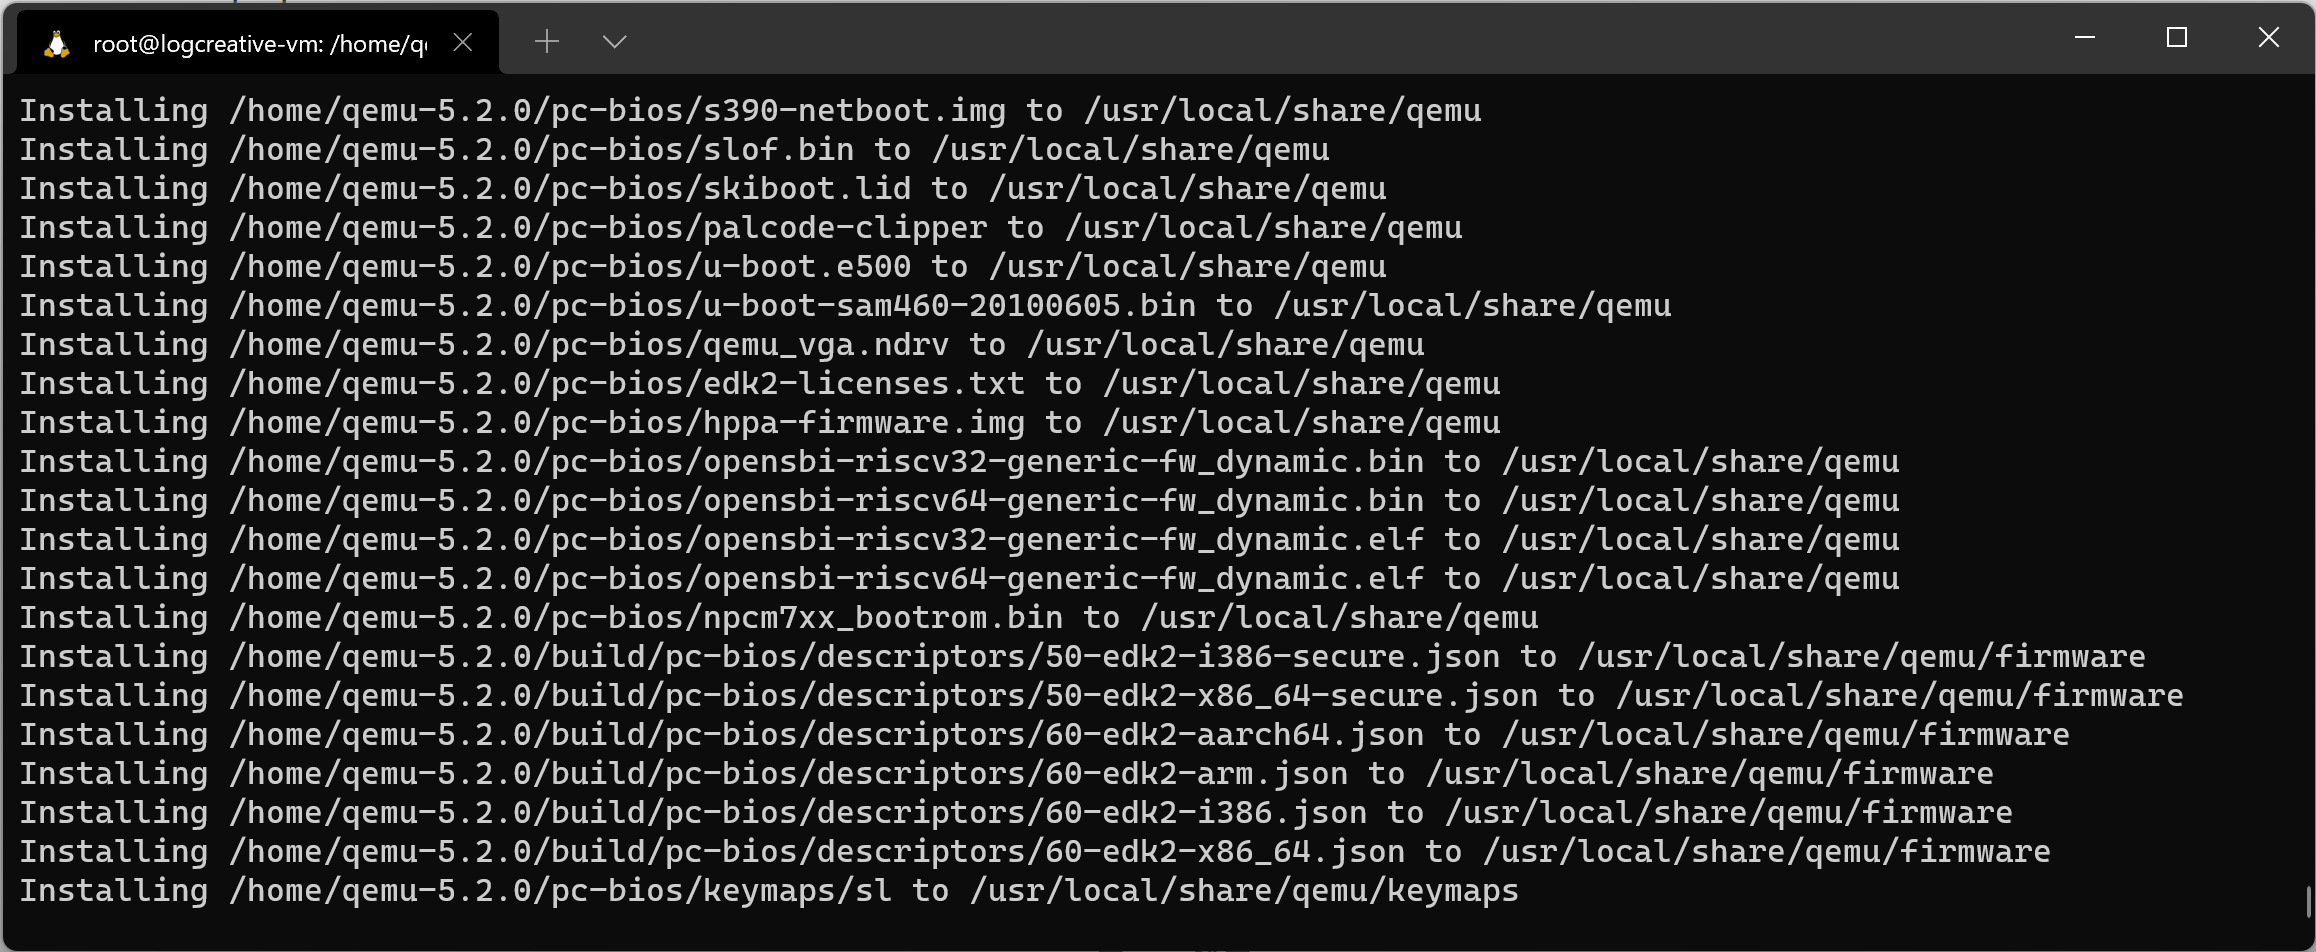
\includegraphics[width=\linewidth]{install}
            \caption{QEMU 安装}\label{fig:install}
        \end{minipage}
    \end{figure}

    % 实际上,这里使用了 git submodule add https://git.sjtu.edu.cn/sjtug/qemu.git
    % 来插入子模块,并且需要使用
    % git submodule update --init --recursive
    % 来刷新内部的子模块
    % 如果出现问题,需要先使用
    % git submodule deinit --all -f
    % 来解除初始化

    \bibliography{ref}
\end{document}